\documentclass[a4paper,german]{scrreprt}

% Uncomment to optimize for double-sided printing.
% \KOMAoptions{twoside}

% Set binding correction manually, if known.
% \KOMAoptions{BCOR=2cm}

% Localization options
\usepackage[german]{babel}
\usepackage[T1]{fontenc}
\usepackage[utf8]{inputenc}

% Enhanced verbatim sections. We're mainly interested in
% \verbatiminput though.
\usepackage{verbatim}

% PDF-compatible landscape mode.
% Makes PDF viewers show the page rotated by 90°.
\usepackage{pdflscape}

% Advanced tables
\usepackage{tabu}
\usepackage{longtable}
\usepackage{dcolumn}
\newcolumntype{d}[1]{D{.}{\cdot}{#1} }

% Fancy tablerules
\usepackage{booktabs}

% Graphics
\usepackage{graphicx}

% Current time
\usepackage[useregional=numeric]{datetime2}

% Float barriers.
% Automatically add a FloatBarrier to each \section
\usepackage[section]{placeins}

% Custom header and footer
\usepackage{fancyhdr}

\usepackage{geometry}
\usepackage{layout}

% Math tools
\usepackage{mathtools}
% Math symbols
\usepackage{amsmath,amsfonts,amssymb}
\usepackage{amsthm}

% SI units
\usepackage{siunitx}
\DeclareSIUnit\Molar{\textsc{m}}

% Chemistry
\usepackage{mhchem}

\DeclarePairedDelimiter\abs{\lvert}{\rvert}

\pagestyle{plain}
% \fancyhf{}
% \lhead{}
% \lfoot{}
% \rfoot{}
% 
% Source code & highlighting
\usepackage{listings}

% Convenience commands
\newcommand{\mailsubject}{2027 - Praktikum Biochemie 1}
\newcommand{\maillink}[1]{\href{mailto:#1?subject=\mailsubject}
                               {#1}}

% Should use this command wherever the print date is mentioned.
\newcommand{\printdate}{\today}

\subject{2027 - Praktikum Biochemie 1}
\title{8 - Renaturierung von Hühnereiweiss-Lysozym}

\author{David Willimann \maillink{david.willimann@students.unibe.ch} - 17-118-977 \\ Michael Senn \maillink{michael.senn@students.unibe.ch} - 16-126-880}

\date{\printdate}

% Needs to be the last command in the preamble, for one reason or
% another. 
\usepackage{hyperref}


\begin{document}
\maketitle

\chapter{Einleitung \& Theorie}

\section{Einleitung}

In diesem Experiment wurde die reversible thermische und chemische
Denaturierung von Hühnereiweiss-Lysozym untersucht. Hierzu wurde einem Ei
Eiweiss entnommen, und die enthaltenen Proteine chemisch und thermisch
denaturiert. Nach erfolgter Renaturierung wurde mittels Photometer die
enzymatische Aktivität gegenüber Zellwänden gemessen, und mit nativem Lysozym
verglichen.

\section{Theorie}

\subsection{Effekt von 6M Harnstoff auf Lysozym}

Harnstoff, als chaotropes Salz, führt zu einer Störung der Wasserstoffbrücken
was - durch Wegfall des hydrophoben Effekts - zur Denaturierung von Lysozym
führt. Da der hydrophobe Effekt jedoch weg fällt, wird das denaturierte Protein
in Lösung übergehen und nicht ausfällen.

\subsection{Effekt der Erwärmung von Lysozym auf \SI[detect-weight]{90}{\celsius}}

Die Erhöhung der kinetischen Energie führt zu einer thermischen Denaturierung
von Lysozym. Durch den weiterhin vorhandenen hydrophoben Effekt wird das
Protein allerdings ausfällen.

Zu beachten ist, dass die kovalenten Disulphidbrücken erhalten bleiben.

\subsection{Effekt der Zugabe von \SI[detect-weight]{0.01}{\Molar} \ce{HCl} zu Lysozym}

Der pH einer 0.01 M \ce{HCl}-Lösung ist gegeben als $\texttt{pH} \approx
-\log_{10}(0.01) = 2$. Solch eine Lösung wird somit jegliche protonierbaren
Seitenketten protonieren. Diese Ladungsverschiebung führt zu einem Wegfall der
ionischen Wechselwirkungen zwischen den Seitenketten, was zu einer
Denaturierung des Lysozyms führt. Da der hydrophobe Effekt weiterhin vorhanden
ist, wird es zu einer Ausfällung des Proteins kommen.

\subsection{Reaktionsmechanismus von Lysozym}

Das aktive Zentrum von Lysozym liegt zwischen einem Aspartat an Stelle 52, und
einer Glutaminsäure an Stelle 35.

In einem ersten Schritt wird die 4-OH Abgangsgruppe des NAG-Restes durch Glu-35
protoniert. Durch das Umklappen der Sessel-Konformation wird die abzuspaltende
Bindung des Substrats schliesslich getrennt. Wasser führt dann dazu, dass die
Bindung zwischen Substrat und Asp-52 des Intermediats aufgehoben wird, und die
ursprüngliche Konformation wiederhergestellt wird. \cite{lys}

Dieser Mechanismus erklärt auch, wieso Lysozym nur in gefaltetem Zustand aktiv
ist - in ungefaltetem Zustand sind Asp-52 und Glu-35 zu weit auseinander, als
dass das Substrat dazwischen binden könnte.

\begin{figure}[h]
	\centering
	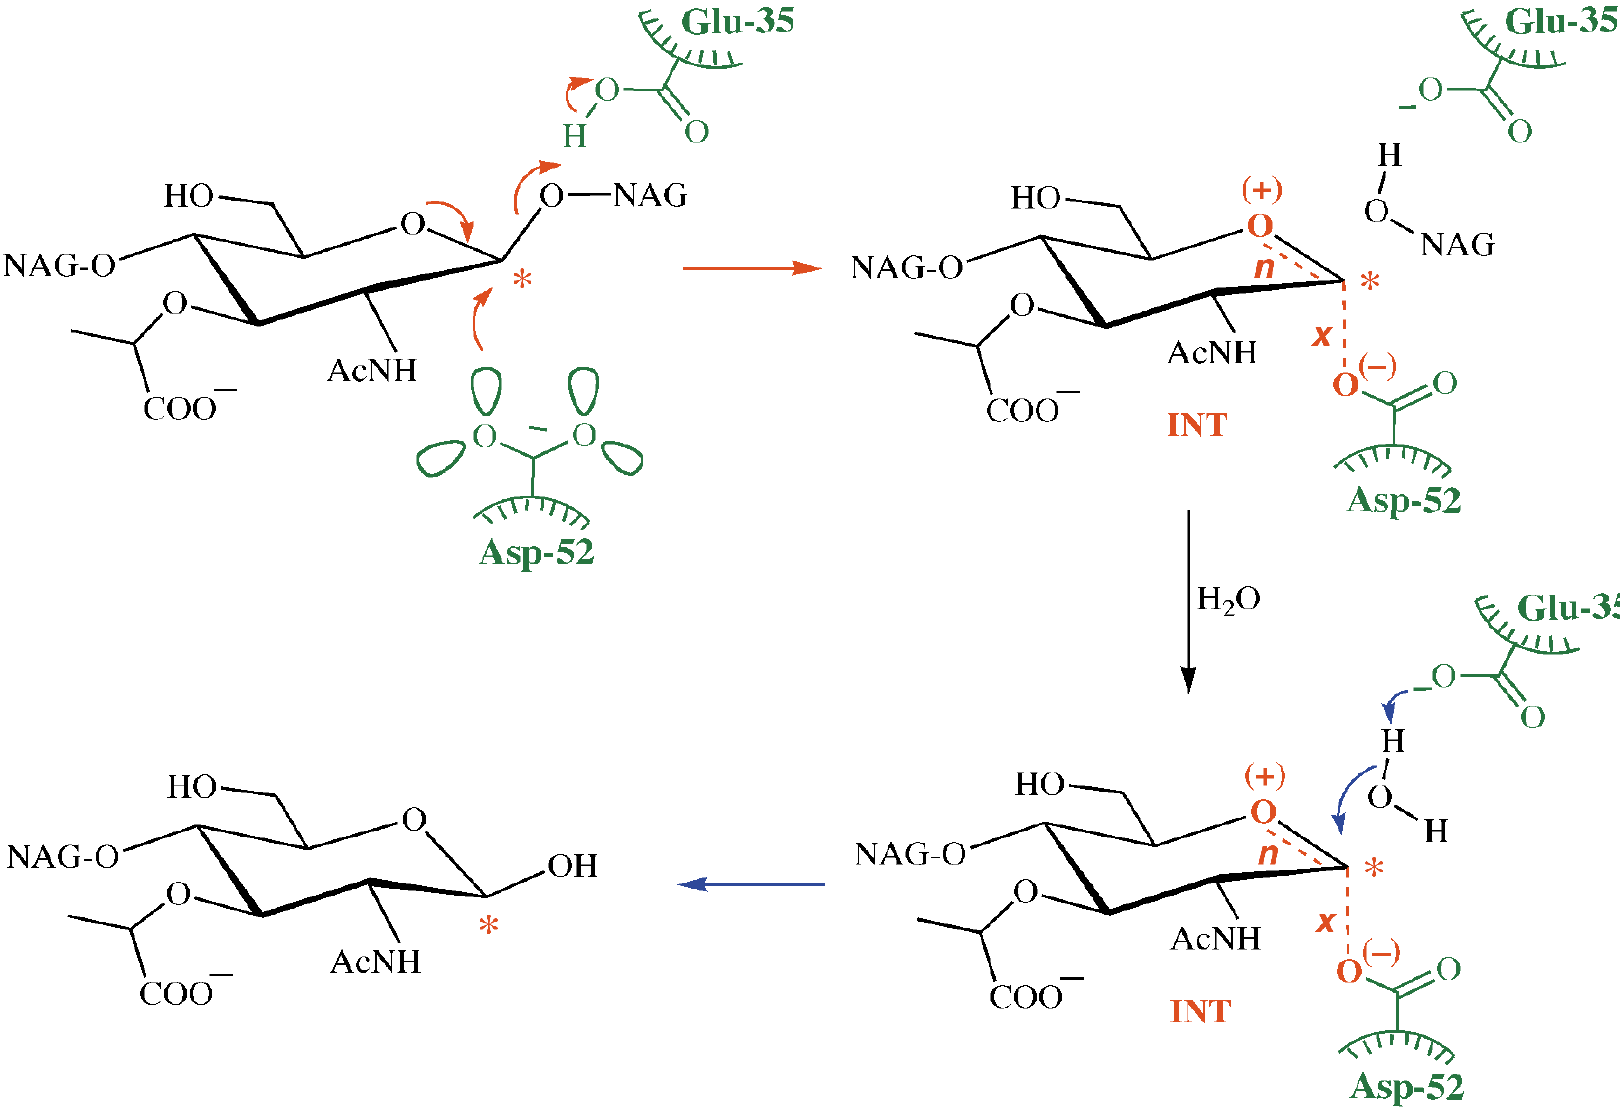
\includegraphics[width=0.9\textwidth]{data/lys_mechanism}
	\caption{Reaktionsmechanismus von Lysozym, aus \cite{lys}}
	\label{fig:lys_mechanism}
\end{figure}

\subsection{Theoretisch mögliche Disulphid-Brücken in Lysozym}

Lysozym hat vier Disulphid-Brücken, und damit acht Cystein-Reste. Damit sind
für die erste Bindung $\binom{8}{2}$, für die zweite $\binom{6}{2}$ etc
Möglichkeiten vorhanden. Da die Reihenfolge der Bindungen keine Rolle spielt,
folgt die totale Anzahl Möglichkeiten als:

\[
	\frac{\binom{8}{2} \binom{6}{2} \binom{4}{2} \binom{2}{2}}{\frac{n}{2}!} = 105
\]

Dies bedeutet, dass Faltungsintermediate so aufgebaut sein müssen, dass die
Bildung der korrekten Disulphid-Brücken bevorzugt wird.

\chapter{Material \& Methoden}

\section{Material}

\begin{itemize}
\item 2 \SI{500}{ml} Bechergläser
\item 1 \SI{100}{ml} Messzylinder
\item 1 Styroporbox, gefüllt mit Eis
\item Dialyseklammern
\item Pipetten \SIrange{10}{100}{\ul}, \SIrange{100}{1000}{\ul}
\item Spritze mit Nadel
\item Magnetrührer
\item Peristaltische Pumpe
\end{itemize}

\section{Chemikalien und Lösungen}

\begin{itemize}
	\item Tris(hexdroxymethyl)amonimethan
	\item EDTA (Triplex III)
	\item Zellwände von Micrococcus
	\item Di-Kaliumhydrogenphosphat
	\item Kalium-dihydrogenphosphat
	\item Guanidine-Hydrochlorid
	\item 1,4 Dithioerythrit (DTE)
	\item Glutathion, oxidiert (GSSG)
	\item Glutathion, reduziert (GSH)
	\item Arginine

	\item 10x TE (Tris-EDTA) \SI{1}{\Molar} Tris
	\begin{itemize}
		\item \SI{1}{\Molar} Tris
		\item \SI{10}{\milli\Molar} Tris
		\item pH: 8.5
	\end{itemize}

	\item Assay-Lösung
	\begin{itemize}
		\item \SI{30}{\milli\Molar} Kaliumphosphat
		\item \SI{0.1}{\percent} (w/v) BSA
		\item \SI{10}{mg} Zellwände Micrococcus lysodeiktikus pro \SI{2.5}{ml}
		\item pH: 7.4
	\end{itemize}

	\item Guanidine-\ce{HCl}
	\begin{itemize}
		\item \SI{8}{\Molar} Guanidine-hydrochlorid
		\item \SI{0.1}{\Molar} Tris
		\item \SI{1}{\milli\Molar} EDTA
	\end{itemize}
	\item GSSG-Puffer
	\begin{itemize}
		\item \SI{0.1}{\Molar} Tris
		\item \SI{1}{\milli\Molar} EDTA
		\item \SI{1}{\milli\Molar} Glutathion, oxidiert (GSSG)
		\item \SI{0.1}{\milli\Molar} Glutathion, reduziert (GSH)
		\item \SI{0.8}{\milli\Molar} Arginine
		\item pH: 8.5
	\end{itemize}
\end{itemize}

\chapter{Methoden}

\section{Vorbereitung Lysozym}

\subsection{Natives Lysozym}

\begin{itemize}
	\item Ei mit Skalpell-spitze ankratzen
	\item \SI{1.3}{ml} Eiweiss entlang der Wand des Eis entnehmen, auf Eis stellen
	\item \SI{0.05}{ml} des entnommenen Eiweiss in \SI{50}{ml} 1x TE lösen,
		auf Eis stellen $\Rightarrow$ natives Lysozym
\end{itemize}

\subsection{Denaturiertes Lysozym}

\begin{itemize}
	\item \SI{0.2}{ml} des entnommenen Eiweiss in \SI{2}{ml}
		Guanidine-\ce{HCl} lösen, bei Raumtemperatur stehen lassen
		$\Rightarrow$ denaturiertes Lysozym
	\item Kurz vor der Aktivitätsmessung in \SI{20}{ml} 1x TE-Puffer unter
		Rühren verdünnen, zwecks Renaturierung.
\end{itemize}

\subsection{Reduziertes Lysozym}

\begin{itemize}
	\item Rest des Eis \SIrange{5}{10}{min} kochen, unter Wasser abkühlen
	\item \SI{1}{g} gekochtes Eiweiss zerdrücken, unter langsamen Rühren in
		\SI{4.5}{ml} Guanidine-\ce{HCl} und \SI{39}{mg} DTE während
		\SI{30}{min} lösen.
	\item Mit Guanidine-\ce{HCl} auf \SI{6.0}{ml} auffüllen.
	\item \SI{1}{ml} der klaren Eiweiss-Lösung entnehmen. Zwecks Entfernung
		von DTE zweimal je eine Stunde gegen \SI{300}{ml}
		Guanidine-\ce{HCl} dialysieren:
	\item Nach zweifacher Dialyse \SI{0.2}{ml} Lösung aus Dialyseschlauch
		entnehmen, und durch sehr langsames Zutropfen von GSSG-Puffer
		auf \SI{20}{ml} verdünnen $\Rightarrow$ reduziertes Lysozym.
\end{itemize}

\section{Aktivitätsmessung}

Folgende Messungen werden durchgeführt:
\begin{itemize}
	\item 2x natives Lysozym
		\begin{itemize}
			\item Morgen: t [min] = 0, 1, 2, \ldots, 10, 19, 20, 29, 30
			\item Nachmittag: t [min] = 0, 1, 2, \ldots, 10, 19, 20, 29, 30
		\end{itemize}
	\item 2x denaturiertes Lysozym
		\begin{itemize}
			\item Erste Messung: t [min] = 0, 1, 2, \ldots, 10, 19, 20, 29, 30, 39, 49, 50
			\item Zweite Messung (40 Minuten nach erster): t [min] = 0, 1, 2, \ldots, 10
		\end{itemize}
	\item 1x reduziertes Lysozym: t [min] = 0, 1, 2, \ldots, 10, 19, 20, 29, 30
\end{itemize}

Zur Vorbereitung der Assays werden \SI{10}{mg} Zellwände in \SI{2.5}{ml}
Assay-Lösung suspendiert, und auf Eis gelagert. Die Assays werden dann wie
folgt hergestellt. Wichtig ist, dass das Lysozym erst kurz vor der Messung
hinzu gegeben wird, da dadurch die Enzym-Aktivität startet:
\\

\begin{tabular}{|l|l|l|l|}
	\hline
	Assay-Lösung          & \SI{100}{\ul} & \SI{100}{\ul} & \SI{100}{\ul} \\
	TE Puffer             & \SI{800}{\ul} & \SI{800}{\ul} & \SI{300}{\ul} \\
	Natives Lysozym       & \SI{100}{\ul} &               &               \\
	Denaturiertes Lysozym &               & \SI{100}{\ul} &               \\
	Reduziertes Lysozym   &               &               & \SI{600}{\ul} \\
	\hline
\end{tabular}
\\

Die Messung der Absorption in Photometer findet bei \SI{578}{nm} statt.  Direkt
vor und zwischen den Messungen müssen die Assays immer wieder gestürzt werden.

\chapter{Resultat}

\section{Messwerte}

\begin{table}[h!]
	\centering
	\begin{tabular}{|l d{3} d{3} d{3} d{3} d{3}|}
		\hline
		Zeit [min] & \multicolumn{1}{c}{$R_1$} & \multicolumn{1}{c}{$D_2$} & \multicolumn{1}{c}{$D_1$} & \multicolumn{1}{c}{$N_2$} & \multicolumn{1}{c|}{$N_1$} \\
		\hline
		0  & 0.393 & 0.346 & 0.413 & 0.392 & 0.372 \\
		\hline
		1  & 0.305 & 0.354 & 0.348 & 0.237 & 0.303 \\
		\hline
		2  & 0.283 & 0.333 & 0.376 & 0.298 & 0.245 \\
		\hline
		3  & 0.24  & 0.349 & 0.371 & 0.298 & 0.313 \\
		\hline
		4  & 0.201 & 0.297 & 0.381 & 0.217 & 0.309 \\
		\hline
		5  & 0.215 & 0.354 & 0.385 & 0.181 & 0.335 \\
		\hline
		6  & 0.156 & 0.305 & 0.359 & 0.231 & 0.316 \\
		\hline
		7  & 0.301 & 0.294 & 0.363 & 0.22  & 0.318 \\
		\hline
		8  & 0.32  & 0.338 & 0.389 & 0.216 & 0.277 \\
		\hline
		9  & 0.303 & 0.249 & 0.297 & 0.232 & 0.333 \\
		\hline
		10 & 0.258 & 0.308 & 0.354 & 0.217 & 0.299 \\
		\hline
		19 & 0.213 &       & 0.248 & 0.234 & 0.277 \\
		\hline
		20 & 0.255 &       & 0.333 & 0.196 & 0.321 \\
		\hline
		29 & 0.632 &       & 0.203 & 0.175 & 0.234 \\
		\hline
		30 & 0.662 &       & 0.28  & 0.133 & 0.199 \\
		\hline
		39 &       &       & 0.298 &       & 0.181 \\
		\hline
		40 &       &       & 0.139 &       & 0.097 \\
		\hline
		49 &       &       & 0.278 &       & 0.269 \\
		\hline
		50 &       &       & 0.34  &       & 0.222 \\
		\hline
	\end{tabular}
	\caption{Absorption bei \SI{578}{nm} von 5 Lysozym-Messreihen.}
	\label{table:1}
\end{table}

In Tabelle \ref{table:1} sind die Rohdaten der fünf Mess-Serien der Lysozym-Lösungen gelistet. Hierbei sind:
\begin{description}
	\item[$N_1$] Erste Messung nativen Lysozyms (Morgen)
	\item[$N_2$] Zweite Messung nativen Lysozyms (Nachmittag)
	\item[$D_1$] Erste Messung denaturierten Lysozyms
	\item[$D_2$] Zweite Messung denaturierten Lysozyms
	\item[$R_1$] Erste Messung reduziertes Lysozyms
\end{description}

Allen Messungen ist gemein, dass sie eine sehr hohe Varianz haben. Potentiell
stammt diese daher, dass die Zellwände in den Assays sich sehr schnell setzten
- und damit der gemessene Absorptionswert stark davon abhängt, ob fünf oder 15
Sekunden vor der Messung das letzte Mal geschüttelt wurde.

Weiterhin sind die letzten zwei Messwerte des reduzierten Lysozyms stark
erhöht. Während der Durchführung war der Parafilm auf der Küvette des
reduzierten Lysozyms nicht satt, was teilweise zu Verlust der Probe führte.
Dies könnte dazu geführt haben, dass gegen Ende der Messreihe nicht mehr
genügend Flüssigkeit in der Küvette war und damit beispielsweise ein Klumpen
Zellwände an der Wand haftete.

Die folgenden Abbildungen stellen den zeitlichen Verlauf der Absorption von Licht der Wellenlänge \SI{578}{nm}, durch die Assays mit nativem (Abbildung \ref{fig:absorption_native}), denaturiertem (Abbildung \ref{fig:absorption_denat}) und reduzierten (Abbildung \ref{fig:absorption_reduced}) Lysozym dar.

Bei nativem und denaturiertem Lysozym zeigt eine lineare Regression einen klare
Abnahme der Absorption über Zeit - ein Resultat des Abbaus der Zellwände durch
das Lysozym. Bei reduziertem Lysozym ist dieser Trend ersichtlich, solange die
beiden letzten Messwerte ignoriert werden (Messreihe ``reduced\_1''). Werden
die beiden letzten Messwerte einbezogen, ist kein solcher Trend ersichtlich
(Messreihe ``reduced\_2'').

\begin{figure}[h]
	\centering
	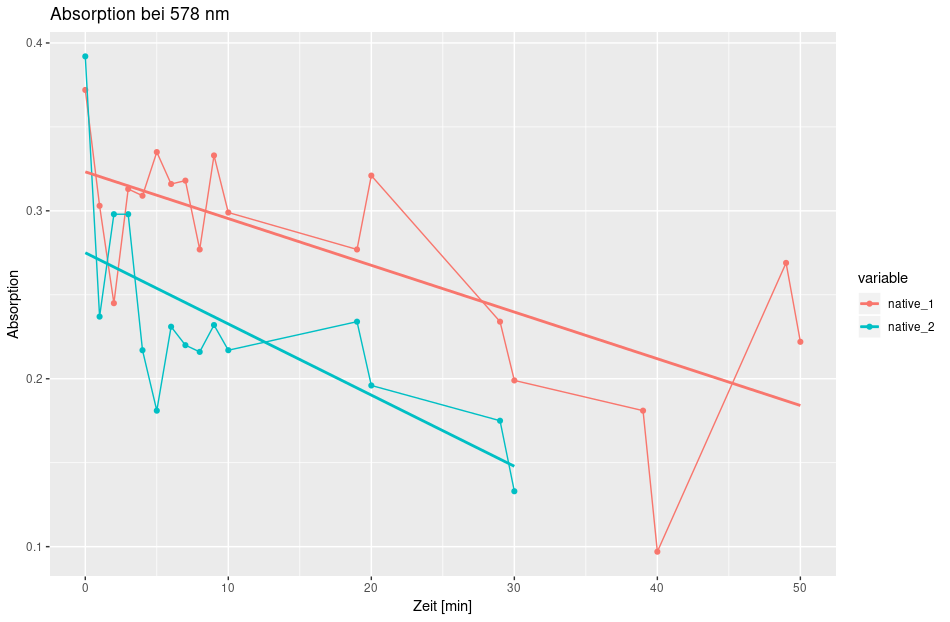
\includegraphics[width=0.9\textwidth]{data/absorption_nativ}
	\caption{Absorption von nativem Lysozym}
	\label{fig:absorption_native}
\end{figure}

\begin{figure}[h]
	\centering
	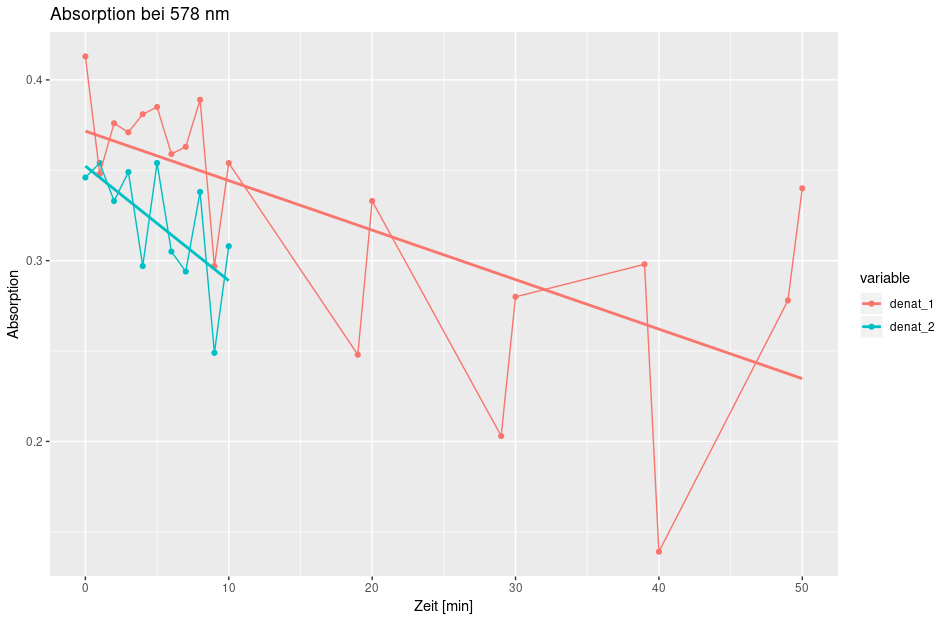
\includegraphics[width=0.9\textwidth]{data/absorption_denat}
	\caption{Absorption von denaturiertem Lysozym}
	\label{fig:absorption_denat}
\end{figure}

\begin{figure}[h]
	\centering
	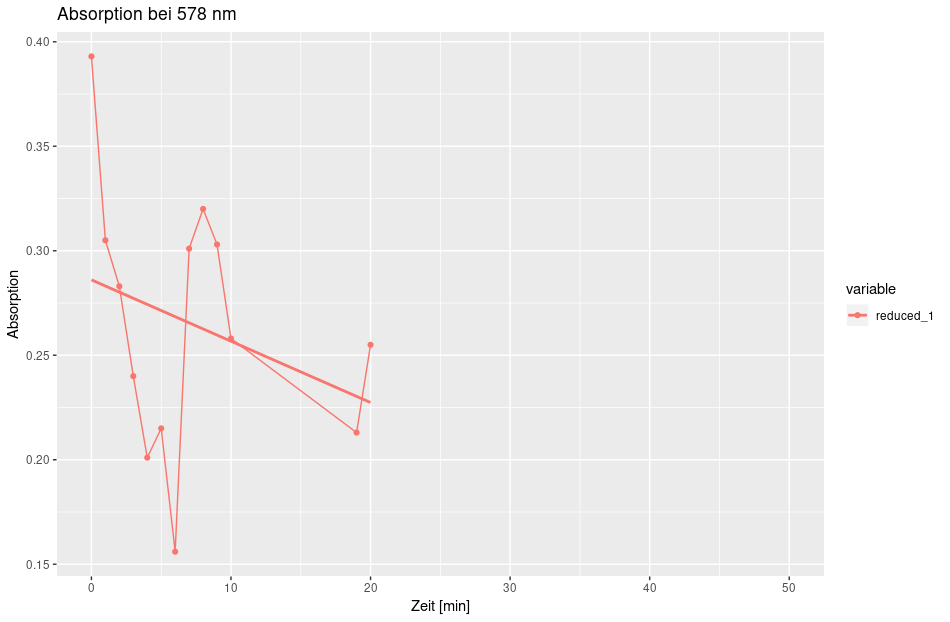
\includegraphics[width=0.9\textwidth]{data/absorption_reduced}
	\caption{Absorption von reduziertem Lysozym}
	\label{fig:absorption_reduced}
\end{figure}

\section{Standardisierte Aktivität}

Um die Messwerte der drei Eiweisslösungen - welche in unterschiedlichem Masse
verdünnt wurden - zu vergleichen, wird die Aktivität definiert als:

\[
	\text{Aktivität} = \frac{\Delta \text{OD}_{578 / \text{min}}}{0.01} \cdot F
\] 

Wobei $\text{OD}_{578 / \text{min}}$ die Veränderung der gemessenen Optischen
Dichte bei \SI{578}{nm} während einer Minute, und $F$ der Verdünnungsfaktor der
Probe - definiert als Inverses der Produkte der einzelnen Verdünnungen - ist.

\subsection{Verdünnungsfaktoren}

Folgende Verdünnungsfaktoren ergeben sich damit:
\begin{itemize}
	\item $F_{\text{nativ}} = \left (
			\frac{\SI{0.05}{ml}}{\SI{50.05}{ml}} \cdot
	                \frac{\SI{100}{ul}}{\SI{1000}{ul}}
		\right )^{-1} = 10010$
	\item $F_{\text{denat}} = \left (
			\frac{\SI{0.2}{ml}}{\SI{2.2}{ml}} \cdot
			\frac{\SI{1}{ml}}{\SI{21}{ml}} \cdot
			\frac{\SI{100}{\ul}}{\SI{1000}{\ul}}
		\right )^{-1} = 2310$
	\item $F_{\text{reduced}} = \left (
			\frac{\SI{1}{ml}}{\SI{6}{ml}} \cdot
			\frac{\SI{0.2}{ml}}{\SI{20}{ml}} \cdot
			\frac{\SI{600}{\ul}}{\SI{1000}{\ul}}
		\right )^{-1} = 1000$
\end{itemize}

\section{Aktivität nativen Lysozyms}

Die durchschnittliche Aktivität von frischem Lysozym innert der ersten 10
Minuten ist gegeben als:

\[
	A_0 = \frac{0.372 - 0.299}{10 \cdot 0.01} \cdot 10010 = 7307.3
\]

\section{Aktivität nativen Lysozyms über Zeit}

Die Aktivität nativen Lysozyms im Laufe der Zeit - als absolute Werte sowohl
als Prozentsatz von $A_0$ - ist gegeben als:
\\

\begin{tabu}{|l|l|l|}
	\hline
	Zeit [min] & Aktivität & Aktivität (\% $A_0$) \\
	\hline
	$A_0$ & 7307.3 & 100\% \\
	10 & 34034 & 466\% \\ 
	20 & -44044 & -603\% \\ 
	30 & 35035 & 479\% \\ 
	\hline
\end{tabu}
\\

Aufgrund der hohen Varianz der Messwerte lässt sich die erwartete Limitierung
der Enzymaktivität aufgrund Substrat-Limitation nicht sehen.

\section{Aktivität natives Lysozym Morgen / Nachmittag}

Die nachstehende Tabelle vergleicht die Enzymaktivität des frischen Lysozyms am
Morgen, mit jener am Nachmittag.
\\

\begin{tabu}{|l|l|l|}
	\hline
	Zeit [min] & Aktivität Morgen & Aktivität Nachmittag \\
	\hline
	$A_0$ & 7307.3 & 17517.5 \\
	10 & 34034 & 38038 \\ 
	20 & -44044 & 42042 \\ 
	\hline
\end{tabu}
\\

Aufgrund der gemessenen Werte scheint die Aktivität des Lysozyms durch gekühlte
Lagerung für einige Stunden nicht gelitten zu haben, was darauf hindeutet, dass
sich gekühltes Lysozym kaum spontan entfaltet. Wegen der hohen Varianz ist
diese Aussage jedoch mit Vorsicht zu geniessen.

\section{Renaturierungsausbeute des denaturierten Eiweiss}

Um nicht aufgrund von Substratlimitation falsche Aussagen zu treffen, sowie um
die hohe Varianz mittels grosser Dichte von Messpunkten zu limitieren, werden
hier nur die $A_0$ Werte - dh mittlere Aktivität innert der ersten 10 Minuten -
verglichen.
\\

\begin{tabu}{|l|l|l|}
	\hline
	Messreihe & $A_0$ & In \% von $A_0$ von $N_1$ \\
	\hline
	$N_1$ & 7307.3 & 100\% \\
	$D_1$ & 1362.9 & 18.7\% \\
	$D_2$ & 877.8 & 12.0\% \\
	\hline
\end{tabu}
\\

Die mittlere Ausbeute von denaturiertem Lysozym liegt somit bei 15.35\%.

\section{Renaturierungsausbeute des reduzierten Eiweiss}

Analog des vorherigen Abschnittes folgt die Renaturierungsausbeute des
reduzierten Eiweiss als:

\begin{align*}
	A_0(N_1) & = 7307.3 \\
	A_0(R_1) & = 1350 \\
	\text{Renaturierungsausbeute} & = \frac{1350}{7307.3} = 0.185
\end{align*}

Die Renaturierungsausbeute von reduziertem Lysozym liegt somit bei 18.5\%.

\section{Vergleich der Renaturierungsausbeuten}

Wie erwartet liegt die enzymatische Aktivität von renaturiertem unter jener von
nativem Lysozym. Folglich kann nicht alles Lysozym im TE-Puffer renaturiert
werden.

Unerwarteter weise liegt $A_0$ des reduzierten Lysozyms allerdings über $A_0$
des denaturierten Lysozyms. Da beim reduzierten Lysozym zusätzlich die
Disulphid-Brücken reduziert wurden, wäre zu erwarten gewesen, dass sich weniger
Lysozym wieder korrekt faltet, und damit enzymatisch aktiv ist.

Dieses Ergebnis wird eine Folge der verschiedenen Fehlerquellen sein, die das
Experiment beeinflusst haben.

\chapter{Fazit}

Aufgrund der extrem hohen Varianz der Messwerte konnten gewisse Erwartungen
nicht nachgewiesen werden. Zusätzlich ist das Vertrauen in die Aussagen die
gemacht wurden relativ klein, da sie potentiell nur ein Resultat von
Schwankungen der Messwerte sind.

Würde das Experiment wiederholt werden, müsste zwingend die Quelle der hohen
Varianz gefunden, und soweit möglich eliminiert werden.

\bibliographystyle{plain}
\bibliography{references}

\end{document}
